\chapter{Underwater granular flows}

\ifpdf
    \graphicspath{{Chapter6/figs/raster/}{Chapter6/figs/pdf/}{Chapter6/figs/}}
\else
    \graphicspath{{Chapter6/figs/vector/}{Chapter6/figs/}}
\fi

\section{Introduction}
Avalanches, landslides, and debris flows are geophysical hazards, which involve 
rapid mass movement of granular solids, water, and air as a single phase 
system. Globally, landslides cause billions of pounds in damage, and thousands 
of deaths and injuries each year. Hence, it is important to understand the 
triggering mechanism and the flow evolution. The momentum transfer between the 
discrete and the continuous phases significantly affects the dynamics of the 
flow 
as a whole~\citep{Topin2012}. Although certain macroscopic models are able to 
capture the simple mechanical behaviours~\citep{Peker2007}, the complex 
physical mechanisms occurring at the grain scale, such as hydrodynamic 
instabilities, 
formation of clusters, collapse, and transport~\citep{Topin2011}, have largely 
been ignored. In particular, when the solid phase reaches a high volume 
fraction, the strong heterogeneity arising from the contact forces between the 
grains, and the hydrodynamic forces, are difficult to integrate into the 
homogenization process involving global averages. 

In order to describe the mechanism of immersed 
granular flows, it is important to consider both the dynamics of the solid 
phase and the role of the ambient fluid~\citep{Denlinger2001}. The dynamics of 
the solid phase alone are insufficient to describe the mechanism of granular 
flows in fluid. It is important to consider the effect of hydrodynamic forces 
that reduce the weight of the solids inducing a transition from dense-compacted 
to dense-suspended flows, and the drag interactions which counteract the 
movement of the solids~\citep{Meruane2010}. Transient regimes characterized by 
a change in the solid fraction, dilation at the onset of flow and the 
development of excess pore-pressure, result in altering the balance between the 
stress carried by the fluid and that carried by the grains, thereby changing 
the overall behaviour of the flow. 

The presence of a fluid phase in a granular medium has profound effects on its 
mechanical behaviour. In dry granular media, the rheology is governed by grain 
inertia and static stresses sustained by the contact network depending on the 
shear-rate and the confining pressure, respectively~\citep{Midi2004}. As the 
fluid inertia and viscosity come into play, complications arise as a result of 
contradictory effects. On one hand, the fluid may delay the onset of
granular flow or prevent the dispersion of the grains by
developing negative pore-pressures~\citep{Pailha2008,Topin2011}. On the other
hand, the fluid lubricates the contacts between grains, enhancing the rate of 
granular flow, but it has a retarding effect at the same time by 
inducing drag forces on the grains. The objective of the present study is to 
understand the differences in the mechanism of flow initiation and kinematics 
between dry and submerged granular flows. In the present study, a coupled 2D 
Lattice-Boltzmann and Discrete Element Method is used to model the fluid-soil 
interactions in  underwater granular flows.  The choice of a 2D geometry has 
the advantage of cheaper computational effort than a 3D case, making it 
feasible to simulate very large systems. The configuration and parameters 
studied in this chapter are presented in~\cref{table:lbm-dem-setup}.



\section{LBM-DEM permeability}

In a 3D granular assembly, the pore spaces between the grains are 
interconnected, whereas in a 2-D assembly, a non-interconnected pore-fluid 
space is formed as the grains are in contact with each 
other. This means that the fluid enclosed between the grains cannot flow 
to the neighbouring pore-spaces.  This results in an unnatural no flow 
condition in 
a 2-D case (\cref{fig:reduction}). In order to overcome this effect, a 
reduction in radius is assumed only during the LBM computation (fluid and fluid 
– solid interaction) steps. The reduced radius of the soil grain, i.e., the 
\textit{hydrodynamic radius r}, allows for interconnected pore space through 
which the pore-fluid can flow similar to the 3D behaviour. The reduction in 
the radius is assumed only during LBM computations, hence this technique has no 
effect on the grain – grain interactions computed using DEM. 

Realistically, the hydrodynamic radius can be varied from $ r = 0.7 R$ to 
$0.95 R$, where \textit{R} is the grain radius. Different permeabilities can be 
obtained for any given initial packing by varying the hydrodynamic radius of 
the grains, without having to change the actual granular packing. This 
introduces a new parameter into the system. In a physical sense, a 
hydrodynamic radius represents the three-dimensional permeability of a 
granular assembly simulated as a two-dimensional geometry. 

\begin{landscape}
\centering
\begin{table}
\centering
\caption{Configurations for LBM-DEM simulations of granular collapse in fluid}
\label{table:lbm-dem-setup}
\begin{tabular}{lcccc}
\toprule
\textbf{Simulations} & \textbf{Aspect ratio} & \textbf{Hydrodynamic radius} & 
\textbf{Packing density (\%)} & \textbf{Slope angle (\si{\degree})}\\ \midrule
\multicolumn{5}{c}{\textbf{Collapse on a horizontal surface}} \\
Effect of initial aspect ratio & 0.2 - 6 & r = 0.7 R &  83 & 0 \\
Effect of permeability & 0.2 - 6 & r = 0.7, 0.75, 0.8, 0.85, 0.9 \& 0.95 R &  
83 & 0 \\
Effect of initial density & 0.8 & r = 0.7, 0.75, 0.8, 0.85, 0.9 \& 0.95 R 
& 79 \& 83 & 0 \\ \midrule
\multicolumn{5}{c}{\textbf{Collapse on an inclined plane}} \\
Effect of initial density & 0.8 & r = 0.9 R & 79 \& 83 & 0, 2.5, 5 \& 7.5 
\\
Effect of permeability & 0.8 & r = 0.7, 0.75, 0.8, 0.85 \& 0.9 R &  79 \& 
83 & 0 \& 5 \\ \midrule
Tall columns & 6 & r = 0.85 R & 79 \& 83 & 0, 2.5, 5 \& 7.5 \\
\bottomrule
\end{tabular}
\end{table}
\end{landscape}

\begin{figure}[tbhp]
\centering
\includegraphics[width=0.45\textwidth]{reduction}
\caption{Schematic representation of the hydrodynamic radius in LBM-DEM 
computation.}
\label{fig:reduction}
\end{figure}

The hydrodynamic 
radius can also be assumed to represent the irregularities on the granular 
surface. The hydrodynamic radius represents asperities on 
the grain surface, which represents a channel for the fluid to flow between the 
grains. 


In order to understand the relation between the hydrodynamic radius and the 
permeability of the granular assembly, horizontal permeability tests are 
performed by varying the hydrodynamic radius as 0.7 R, 0.75 R, 0.8 R, 0.85 R, 
0.9 R and 0.95 R. A square sample of 
$50~\si{\mm} 
\times 50~\si{\mm}$ filled with poly-disperse ($d_{max}/d_{min} = 1.8$) grains 
having a mean diameter of 1.7~\si{\mm} is used to determine the relation 
between the hydrodynamic radius and the permeability. Dirichlet boundary 
condition (discussed in~\cref{sec:lbm_bc}), i.e., density constraint,  
is applied along the left and the right boundaries of the sample. The fluid 
density on the left boundary is increased in small steps ($10^{-4} \Delta P$), 
while a constant density is maintained on the right boundary. This results in a 
pressure gradient causing 
the fluid to flow (\cref{fig:perm}) through the pore-space. 

 
\begin{figure}[tbhp]
	\centering
	\begin{subfigure}[b]{0.475\textwidth}
		\centering
		\includegraphics[width=\textwidth]{Pressure}
		\caption{Pressure gradient in the granular assembly}
		\label{fig:pressure}
	\end{subfigure}
	\begin{subfigure}[b]{0.475\textwidth}
		\centering
		\includegraphics[width=0.8\textwidth]{Velocity}
		\caption{Horizontal flow due to pressure gradient}
		\label{fig:velocity}
	\end{subfigure}
	\caption{Evaluation of the horizontal permeability for a 
	hydrodynamic radius of 0.7 R.}
	\label{fig:perm}
\end{figure}


For a given hydrodynamic radius, the 
pressure gradient $\Delta P$ is varied to obtain different flow rates. Probing 
the fluid space showed a Poiseuille flow behaviour between the grains. The flow 
is still within the Darcy's laminar flow regime, which is verified by the 
linear slope between the pressure gradient and the mean flow velocity 
(\cref{fig:permeability}). From the mean flow velocity (\textit{v}), 
the transverse permeability (\textit{k}) of the sample is computed as:
%
\begin{equation}
k=v\cdot\mu\cdot\frac{\Delta x}{\Delta P} \,,
\end{equation}
%
where $\mu$ is the dynamic viscosity of the fluid (\si{\Pa\s}), $\Delta x$ is 
the thickness of the bed of porous medium \si{\m}, and $\Delta P$ is the 
applied pressure difference \si{\Pa}. It can be observed that with increase in 
the hydrodynamic radius the permeability decreases, i.e., the slope of the mean 
flow velocity to the pressure gradient decreases. At very low pressure 
gradients 
($\Delta P \le 0.1$), both 0.9 R and 0.95 R have no flow. Even at 
higher pressure gradients, a hydrodynamic radius of $r = 0.95 R$ shows almost 
no 
flow behaviour. A high value of hydrodynamic radius $r > 0.95 R$ 
results in unnatural flow/no-flow behaviour. Hence in the present study, a 
hydrodynamic radius in the range of 0.7 to 0.95 R is adopted.

\begin{figure}[htpb]
\centering
\includegraphics[width=0.95\textwidth]{Permeability}
\caption{Variation of the mean flow velocity with pressure gradient for 
different hydrodynamic radius.}
\label{fig:permeability}
\end{figure}


Increase in the hydrodynamic radius from 0.7 to 0.95 reduces the porosity from 
0.60 to 0.27. The permeability computed from LB – DEM method is verified by 
comparing it with the analytical solution. One of the widely used analytical 
solution for permeability is the Carman – Kozeny equation (CK Model), 
which is based on the Poiseuille's flow through a pipe and is mainly used for 
3D, homogeneous, isotropic, granular porous media at moderate porosities. In 
the present study, a modified Carman – Kozeny equation that takes into account 
of the micro-structure of the fibres and that is valid in a wide range of 
porosities is adopted~\citep{Yazdchi2011}. The normalized permeability is 
defined as
\begin{equation}
\frac{k}{d^2} = \frac{\epsilon}{\psi_{CK}(1-\epsilon)^2} \,.
\end{equation}
%
In the CK model, the hydraulic diameter $D_h$ , is expressed as a function of 
measurable quantities: porosity and specific surface area
%
\begin{align}
D_h & = \frac{4\epsilon V}{S_v}=\frac{\epsilon d}{(1 - \epsilon)} \,, \\
a_v & = \frac{\mbox{grain surface}}{\mbox{grain volume}} = 
\frac{S_v}{(1-\epsilon V)} = \frac{4}{d} \,,
\end{align}
%
where $S_v$ is the total wetted surface, and $a_v$ is the specific surface 
area. The above value of $a_v$ is for circles (cylinders) - for spheres $a_v = 
6/d$. $\psi_{CK}$ is the empirically  measured CK factor, which represents both 
the shape factor and the deviation of flow direction from that in a duct. It is 
approximated for randomly packed beds of spherical grains. The variation of 
normalized permeability with porosity, obtained by varying the radius from 0.7 R
to 0.95 R, is presented in~\cref{fig:Carman}. The permeability values obtained 
from LBM - DEM simulations are found to match the qualitative trend of the 
Carman-Kozeny equation. The LB – DEM permeability curve lies between the 
permeability curves for spherical and cylindrical grain arrangements implying a 
better simulation of three-dimensional permeability using a 2D granular 
assembly. Thus using a hydrodynamic radius, realistic 3D fluid - grain 
interactions can be simulated in a 2D geometry.

\begin{figure}[htpb]
\centering
\includegraphics[width=0.9\textwidth]{Carman}
\caption{Relation between permeability and porosity for 
different hydrodynamic radius and comparison with the analytical solution.}
\label{fig:Carman}
\end{figure}


\section{Granular collapse in fluid}

The collapse of a granular column, which mimics the
collapse of a cliff, has been extensively studied in the case of
dry granular material, when the interstitial fluid plays no
role (\cref{sec:dry_granular_column}). The problem of the granular collapse 
in a liquid, which is of importance for submarine landslides, has attracted 
less attention~\citep{Rondon2011}.~\citet{Thompson2007} 
observed that the presence of liquid dramatically changes the way a granular 
column collapses compared to the dry case. The destabilization of a granular 
pile strongly depends on the initial volume fraction. For dense 
packings the granular flow is localized at the free surface of the pile, 
whereas for loose packings the destabilization occurs in the bulk of the
material and has a parabolic profile~\citep{Bonnet2010,Topin2011,Iverson2000}. 

\subsection{LBM-DEM set-up}

In the present study, the collapse of a granular column in fluid is studied 
using 2D LBM - DEM. The effect of initial aspect ratio on the run-out behaviour 
is investigated. The flow kinematics are compared with the dry and buoyant 
granular collapse to understand the influence of hydrodynamic forces and 
lubrication on the run-out. Unlike dry column, the permeability and the 
initial volume fraction are expected to have a significant influence on the 
flow dynamics. Hence the effect of these parameters on the run-out behaviour 
is investigated.

The granular column collapse set-up in fluid is very similar to the dry 
granular column collapse. A rectangular channel of length $L_0$ and height 
$H_0$ is filled with poly-dispersed discs, $d_{max}/d_{min} = 1.8$  
(\Cref{fig:geometry}). Once the DEM soil grains reach equilibrium in the dry 
condition, the granular sample is then placed in the fluid domain simulated 
using LBM. The LBM-DEM set-up of a granular column with an aspect ratio 
\textit{a} of 6 in fluid is shown in~\cref{fig:LBMgeometry}. The fluid has a 
density of 
\SI{1000}{\kg\per\cubic\meter}  and a kinematic viscosity of 
\SI{1e-6}{\square\meter\per\second}. The gate supporting the right-hand 
side 
boundary of the granular column is opened allowing the column to collapse and 
flow in a fluid. The final run-out distance is measured as $L_f$ and 
final collapse height as $H_f$. The collapse takes place on a horizontal 
surface. The initial aspect ratio of the column is varied as 0.2, 0.4, 0.6, 
0.8, 1, 2, 4 and 6. 

\begin{figure}[htpb]
\centering
\begin{subfigure}[b]{0.975\textwidth}
\centering
\includegraphics[width=\columnwidth]{geometry}
\caption{Schematic view of underwater granular collapse set-up.}
\label{fig:geometry}
\end{subfigure} \\

\begin{subfigure}[b]{0.975\textwidth}
\centering
\includegraphics[width=\columnwidth]{a6/ini_a6_geom}
\caption{LBM-DEM simulation of underwater granular collapse set-up (\textit{a} 
= 6).}
\label{fig:LBMgeometry}
\end{subfigure}
\caption{Underwater granular collapse set-up.}
\label{fig:LBM_Scheme_geometry}
\end{figure}


The cumulative $\beta$ distribution is adopted to generate grains with 
$d_{max}$ and $d_{min}$ as 2.2~\si{\mm} and 1.25~\si{\mm}, respectively. The 
soil column is modelled using $\sim 2000$ discs of density 
\SI{2650}{\kg\per\cubic\meter} and a contact friction angle of 
\SI{26}{\degree}. A linear-elastic contact model is used in the
DEM simulations. The granular assembly has a packing fraction of $83\%$. The 
critical time step for DEM is computed based on the local 
contact natural frequency and damping ratio. A sub-cycling time integration is 
adopted in DEM (\cref{sec:coupled_lbm_dem}). A fluid flow (LBM) time step 
of $\Delta t = 2.0\times 10^{-5}$\si{\s} is determined based on the viscosity 
and the relaxation parameter $\tau = 0.506$. An integer ratio $n_s$, between 
the fluid flow time step $\Delta t$ and the DEM time step $\Delta t_D$ is 
determined as 15, i.e., every LBM iteration involves a sub-cycle of 15 DEM 
iterations.

In order to capture the realistic physical behaviour of the fluid – grain 
systems, it is essential to model the boundary condition between the fluid and 
the grain as a non-slip boundary condition, i.e. the fluid near the grain 
should have similar velocity as the grain boundary. The solid grains inside the 
fluid are represented by lattice nodes. The discrete nature of the lattice 
results in a stepwise representation of the surfaces (\cref{fig:LBM-DEM}), 
which are otherwise circular, hence sufficiently small lattice spacing $h$ is 
required. The smallest DEM grain in the system controls the size of the 
lattice. In the present study, a very fine discretisation of $d_{min}/h = 10$ 
is adopted, i.e., the smallest grain with a diameter $d_{min}$ in the system is 
discretised into 100 lattice nodes ($ 10h \times 10h$). This provides a very 
accurate representation of the interaction between the solid and the fluid 
nodes.  A hydrodynamic radius of 0.7 R is adopted during the LBM computations. 
The fluid pressure on the top and right boundaries are maintained constant. 
Hence, any pressure wave that is generated during the collapse is absorbed in 
the boundary. Frictional boundary constraint is applied along the bottom 
boundary.

\begin{figure}[htpb]
\centering
\includegraphics[width=0.97\textwidth]{LBM-DEM}
\caption{Discretisation of solid grains in LBM grid. Shows the step-wise 
representation of circular disks in the lattice.}
\label{fig:LBM-DEM}
\end{figure}


\subsection{Collapse in fluid: Flow evolution}
\label{sec:collapse_fluid_evolution}
Two-dimensional plane-strain LBM-DEM simulations of granular column 
collapse are performed by varying the initial aspect ratio of the column from 
0.2 to 6. The normalized final run-out distance is measured as $\Delta L = 
(L_{\textit{f}}-L_{\textit{0}})/L_{\textit{0}}$. Similar to the dry granular 
collapse, the duration of collapse is normalised with a critical time $\tau_c 
= \sqrt{H/g}$, where $H$ is the initial height of the granular column and 
\textit{g} is 
the acceleration due to gravity.  Dry and buoyant analyses of granular column 
collapse are also performed to understand the effect of hydrodynamic forces on 
the run-out distance.

Snapshots of the flow evolution of a granular column collapse with an initial 
aspect ratio of 0.4 are shown in~\cref{fig:a04_snapshots}. The failure begins 
at the toe end of the column, and the fracture surface propagates into the 
column at an angle of about $50\si{\degree}$, similar to the dry column 
collapse. For the 
short column, the failure is due to collapse of the flank. Once the material 
is destabilised, the granular mass interacts with the surrounding fluid 
resulting in formation of turbulent vortices. These vortices interact with the 
grains at the surface resulting in irregularities on the free surface. Force 
chains can be observed in the static region of collapse, which indicates the 
flow can be described using a continuum theory. As the granular material ceases 
to flow, 
force chains develop at the flow front, revealing consolidation of the granular 
mass resulting in an increase in the shear strength. 

\begin{figure}
\begin{subfigure}[b]{0.95\textwidth}
	\centering
    \includegraphics[width=0.95\textwidth]{a04/a04_0}
    \caption{$t = 0\tau_c$}
    \label{fig:a04_0}
\end{subfigure}
\\
\begin{subfigure}[b]{0.95\textwidth}
	\centering
    \includegraphics[width=0.95\textwidth]{a04/a04_tc}
    \caption{$t = 1\tau_c$}
    \label{fig:a04_tc}
\end{subfigure}
\\
\begin{subfigure}[b]{0.95\textwidth}
	\centering
    \includegraphics[width=0.95\textwidth]{a04/a04_3tc}
    \caption{$t = 3\tau_c$}
    \label{fig:a04_3tc}
\end{subfigure}
\\
\begin{subfigure}[b]{0.95\textwidth}
	\centering
    \includegraphics[width=0.95\textwidth]{a04/a04_6tc}
    \caption{$t = 6\tau_c$}
    \label{fig:a04_6tc}
\end{subfigure}
\\
\begin{subfigure}[b]{0.95\textwidth}
	\centering
    \includegraphics[width=0.95\textwidth]{a04/a04_8tc}
    \caption{$t = 8\tau_c$}
    \label{fig:a04_8tc}
\end{subfigure}

\caption[Flow evolution of a granular column collapse in fluid (a = 0.4)]{Flow 
evolution of a granular column collapse in fluid (a = 0.4). Shows 
the velocity profile of fluid due to interaction with the grains (red - higher 
velocity).}
\label{fig:a04_snapshots}
\end{figure}


The evolution of run-out with time for a short column (a = 0.4) is presented 
in~\cref{fig:Runout_a04f}. The dry column exhibits longer run-out distance in 
comparison to the submerged column. The collapse of a dry column using DEM 
represents a collapse in a vacuum, without any influence of drag forces or 
viscosity of air. A LBM-DEM simulation of a granular column collapse using the 
kinematic viscosity of air is performed to compare the dry column with the 
collapse in air. Although the effect of viscous drag can be observed in the 
collapse in the air, both the ``dry'' condition and the 
collapse in air show almost the same run-out behaviour. However, the collapse 
in fluid (water) results in a much shorter run-out distance. The granular mass 
in fluid has the buoyant mass, in contrast to the dry density. A dry granular 
collapse with the buoyant unit weight also 
exhibits longer run-out behaviour than the collapse in fluid. However, due to 
decrease in the initial potential energy, the run-out observed in the buoyant 
condition is shorter than the dry condition. The column collapse in fluid takes 
longer to evolve, which might be due to the development 
of large negative pore water pressure that is generated during the shear 
failure along the fracture surface. This large negative pore-pressure has to be 
dissipated before the granular mass, above the fracture surface, can collapse 
and flow. The shorter run-out distance in the fluid case, in comparison with 
the dry and buoyant conditions, shows that the collapse in fluid is 
significantly affected by the hydrodynamic drag forces acting on the soil 
grains. The evolution of height $H/L$ is presented in~\cref{fig:Height_a04f}. Since the 
failure of the 
column is only at the flank, the central static region remains unaffected. 
Hence, the final height of the column is the same in dry and submerged 
conditions.

\begin{figure}[htpb]
\centering
\begin{subfigure}[t]{0.9\textwidth}
\includegraphics[width=\textwidth]{Runout_a04f}
\caption{Evolution of run-out with time}
\label{fig:Runout_a04f}
\end{subfigure}

\begin{subfigure}[t]{0.9\textwidth}
\centering
\includegraphics[width=\textwidth]{Height_a04f}
\caption{Evolution of height with time}
\label{fig:Height_a04f}
\end{subfigure}
\caption{Evolution of height and run-out with time for a column collapse in 
fluid (a = 0.4).}
\label{fig:a04_run_height}
\end{figure}

The evolution of the normalised kinetic energy with time for a column with an 
initial aspect ratio of 0.4 is shown in~\cref{fig:a04f_energy}. It can be 
observed that the peak kinetic energy is attained later in the submerged 
condition than the dry collapse. This can be attributed to the time required to 
overcome the negative pore-pressure generated during the shear along the 
fracture surface. For short columns the critical time $\tau_c$ is controlled by 
the vertical kinetic energy. The amount of kinetic energy in submerged case is 
significantly lower than the dry condition. Also, the potential energy 
evolution (\cref{fig:PE_a04f}) shows a significant influence of the 
hydrodynamic forces on the amount of material destabilised during the collapse. 
The drag forces on the soil grains reduce and slow down the amount of material 
that undergo collapse resulting in a shorter run-out distance for short 
columns. 
\begin{figure}
\centering
\begin{subfigure}[t]{0.8\textwidth}
	\centering
    \includegraphics[width=\textwidth]{KE_a04f}
    \caption{Evolution of the total kinetic energy.}
    \label{fig:KE_a04f}
\end{subfigure}
\\
\begin{subfigure}[t]{0.95\textwidth}
	\centering
    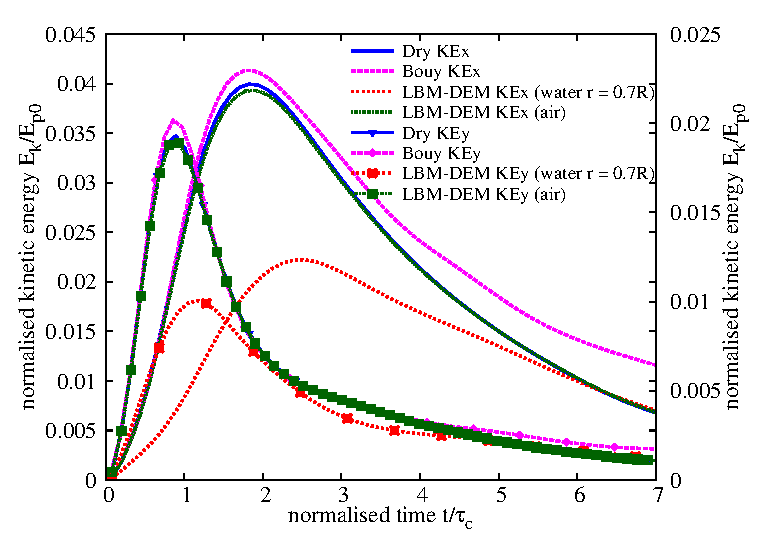
\includegraphics[width=\textwidth]{KExy_a04f}
    \caption{Evolution of horizontal and vertical kinetic energies.}
    \label{fig:KExy_a04f}
\end{subfigure}
\caption{Evolution of kinetic energies with time for a granular column collapse 
in fluid (a = 0.4)}
\label{fig:a04f_energy}
\end{figure}

\begin{figure}
	\centering
    \includegraphics[width=0.9\textwidth]{PE_a04f}
    \caption{Evolution of the potential energy with time for a granular column 
    collapse in fluid (a = 0.4)}
    \label{fig:PE_a04f}
\end{figure}


Snapshots of the flow evolution of a granular column collapse with an initial 
aspect ratio of 4 is shown in~\cref{fig:a4_snapshots}. For a tall column, the 
collapse mechanism changes. The entire column is involved in the collapse. The 
height of the static region, which is below the fracture surface, is shorter 
than the total height of the column. This results in a free-fall of grains 
above the fracture surface. As the grains experience free-fall they interact 
with the surrounding fluid. However, no vortices are observed during the 
initial stage of collapse. In the second phase, when the grains reach the base, 
the vertical acceleration gained during the free-fall is converted into
horizontal velocity. As the grains are ejected horizontally, the free 
surface of the granular mass interacts with the fluid resulting in the 
formation of turbulent vortices. Unlike short columns, these vortices have 
significant 
influence on the mass distribution along the run-out. Heaps of granular 
material can be observed in front of each vortex. The number of vortices 
formed during a collapse is found to be proportional to the amount of material 
destabilised, i.e., the length of free-surface interacting with the fluid 
influences the number of vortices generated during the collapse. The 
reappearance of force chains at $t = 6\tau_c$ and $8\tau_c$ indicates the 
granular mass is consolidating resulting in an increase in the shear strength. 

\begin{figure}
\begin{subfigure}[b]{0.975\textwidth}
	\centering
    \includegraphics[width=\textwidth]{a4/a4_0}
    \caption*{$t = 0\tau_c$}
    \label{fig:a4_0}
\end{subfigure}
\\
\begin{subfigure}[b]{0.975\textwidth}
	\centering
    \includegraphics[width=\textwidth]{a4/a4_tc}
    \caption*{$t = 1\tau_c$}
    \label{fig:a4_tc}
\end{subfigure}
\\
\begin{subfigure}[b]{0.975\textwidth}
	\centering
    \includegraphics[width=\textwidth]{a4/a4_3tc}
    \caption*{$t = 3\tau_c$}
    \label{fig:a4_3tc}
\end{subfigure}
\end{figure}
\begin{figure}
\ContinuedFloat
\begin{subfigure}[b]{0.975\textwidth}
	\centering
    \includegraphics[width=\textwidth]{a4/a4_6tc}
    \caption*{$t = 6\tau_c$}
    \label{fig:a4_6tc}
\end{subfigure}
\\
\begin{subfigure}[b]{0.975\textwidth}
	\centering
    \includegraphics[width=\textwidth]{a4/a4_8tc}
    \caption*{$t = 8\tau_c$}
    \label{fig:a4_8tc}
\end{subfigure}

\caption[Flow evolution of a granular column collapse in fluid (a = 4)]{Flow 
evolution of a granular column collapse in fluid (a = 4). Shows 
the velocity profile of fluid due to interaction with the grains (red - higher 
velocity).}
\label{fig:a4_snapshots}
\end{figure}

The time evolution of the run-out and the height of a tall column (a = 4) is 
presented in~\cref{fig:Runout_a4f} and~\cref{fig:Height_a4f}, respectively. 
Similar to the short column, the run-out observed in the dry condition is much 
longer than that observed in the submerged condition. Also, the evolution of 
run-out is slower in the case of submerged condition, which indicates the 
influence of drag force on the run-out evolution. The height of the column is 
strongly influenced by the hydrodynamic forces 
(\cref{fig:Height_a4f,fig:PE_a4f}), which reduces the amount of material 
destabilised during the collapse.  

\begin{figure}[htpb]
\centering
\begin{subfigure}[t]{0.9\textwidth}
\centering
\includegraphics[width=\textwidth]{Runout_a4f}
\caption{Evolution of run-out with time}
\label{fig:Runout_a4f}
\end{subfigure}

\begin{subfigure}[t]{0.9\textwidth}
\centering
\includegraphics[width=\textwidth]{Height_a4f}
\caption{Evolution of height with time}
\label{fig:Height_a4f}
\end{subfigure}
\caption{Evolution of run-out and height with time for a column collapse in 
fluid (a = 4)}
\label{fig:a4f}
\end{figure}

\begin{figure}
	\centering
    \includegraphics[width=0.9\textwidth]{PE_a4f}
    \caption{Evolution of the potential energy with time for a granular column 
    collapse in fluid (a = 4)}
    \label{fig:PE_a4f}
\end{figure}

The evolution of kinetic energies with time for an initial aspect ratio 4 is 
presented in~\cref{fig:a4f_energy}. Even during the free-fall stage, the peak 
vertical kinetic energy is delayed in the case of fluid, which shows the 
influence of viscosity on the flow evolution. Almost half of the kinetic energy 
that is available in the case of dry granular collapse is dissipated through 
the drag forces experienced by the grains. This shows that the influence of 
viscous drag on the run-out evolution is significantly higher than the effect 
of lubrication.

\begin{figure}
\centering
\makebox[\linewidth][c]{
\begin{subfigure}[t]{0.8\textwidth}
	\centering
    \includegraphics[width=\textwidth]{KE_a4f}
    \caption{Evolution of the total kinetic energy}
    \label{fig:KE_a4f}
\end{subfigure}
}\\
\makebox[\linewidth][c]{
\begin{subfigure}[t]{0.95\textwidth}
	\centering
    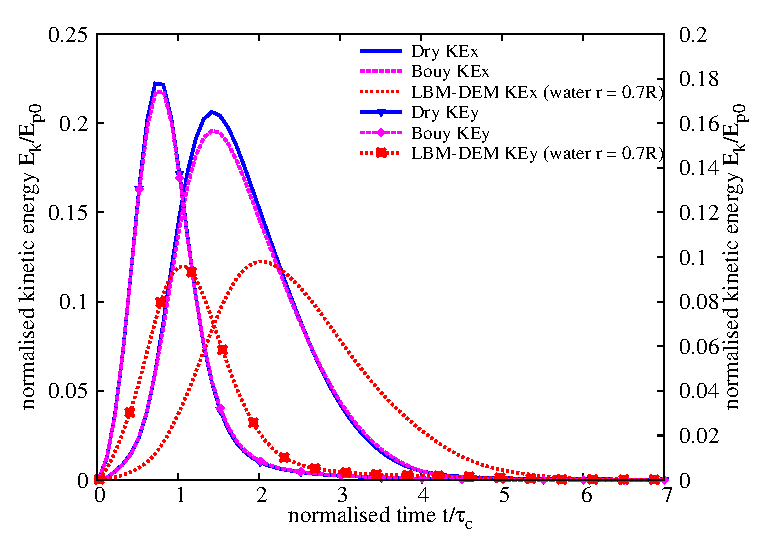
\includegraphics[width=\textwidth]{KExy_a4f}
    \caption{Evolution of horizontal and vertical kinetic energies}
    \label{fig:KExy_a4f}
\end{subfigure}
}
\caption{Evolution of kinetic energies with time for a granular column collapse 
in fluid (a = 4)}
\label{fig:a4f_energy}
\end{figure}

The final 
run-out distance as a function of the initial aspect ratio of the column is 
presented in~\cref{fig:runoutf}. For all aspect ratios, the run-out observed in 
the dry case is significantly higher than the submerged condition. For short 
columns, the run-out distance is found to be have a linear relationship with 
the initial aspect ratio of the column.  A power law 
relation is observed between the run-out and the initial aspect ratio of the 
column.
%
\begin{align}
\frac{L_{\textit{f}}-L_{\textit{0}}}{L_{\textit{0}}} \propto 
\begin{cases}
a, &\qquad \textit{a}\lesssim 2.7 \\
a^{2/3}, &\qquad \textit{a} \gtrsim 2.7 \\
\end{cases}
\end{align}
%
The normalised final height as a function of the initial aspect ratio 
of the column is presented in~\cref{fig:heightf}. It can be observed that the 
final collapse height is much higher in the submerged condition than the dry 
condition. The drag force on the granular column reduces the amount of 
collapse, resulting in a shorter run-out distance. The drag force seems to have 
a predominant influence on the run-out behaviour than the lubrication effect in 
fluid. 


\begin{figure}
	\centering
\begin{subfigure}[t]{0.9\textwidth}
	\centering
	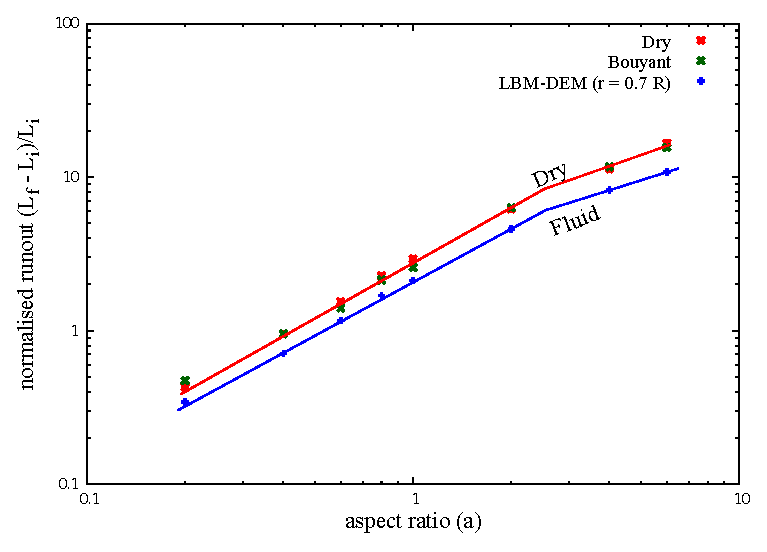
\includegraphics[width=\textwidth]{runoutf}
	\caption{Normalised final run-out distance for columns with different 
	initial aspect ratios. Comparison of dry and submerged granular column 
	collapse.}
	\label{fig:runoutf}
\end{subfigure}\\
\begin{subfigure}[t]{0.9\textwidth}
	\centering
	\includegraphics[width=\textwidth]{Heightf}
	\caption{Normalised final collapse height for columns with different 
	initial aspect ratios. Comparison of dry and submerged granular column 
	collapse.}
	\label{fig:heightf}
\end{subfigure}
	\caption[Comparison of run-out and height between dry and submerged 
	collapse for columns with different initial aspect ratios]{Normalised final 
	collapse run-out and height for columns with 
	different initial aspect ratios.}
	\label{fig:height_runout_fluid}
\end{figure}


\clearpage

\subsection{Effect of permeability}
\citet{Topin2011} observed development of large negative pore-pressure during 
dispersion of grains. The rate of dissipation of the negative pore-pressure is 
directly proportional to the permeability of the granular assembly. In the 
previous section, the evolution of run-out with the initial aspect ratio is 
studied using a constant hydrodynamic radius r = 0.7 R. In order to understand 
the effect of permeability on the run-out behaviour, the hydrodynamic radius 
\textit{r} 
is varied from 0.7 R to 0.95 R for all aspect ratios. Increase in 
the hydrodynamic radius decreases the permeability of the granular assembly 
resulting in a longer duration for the dissipation of negative pore-pressure. 

The normalised run-out for different hydrodynamic radii for a granular column 
with an initial aspect ratio of 0.8 are presented 
in~\cref{fig:Runout_a08_dense}. The run-out increases with decrease in the 
permeability, which is equivalent to an increase in the hydrodynamic radius. 
An increase in the hydrodynamic radius from 0.7 to 0.95 R increases the 
normalised run-out by 25\%. However, even under a very low permeability 
condition (r = 0.95 R), the run-out observed in fluid is shorter than the dry 
and the buoyant conditions. 

\begin{figure}[htpb]
\centering
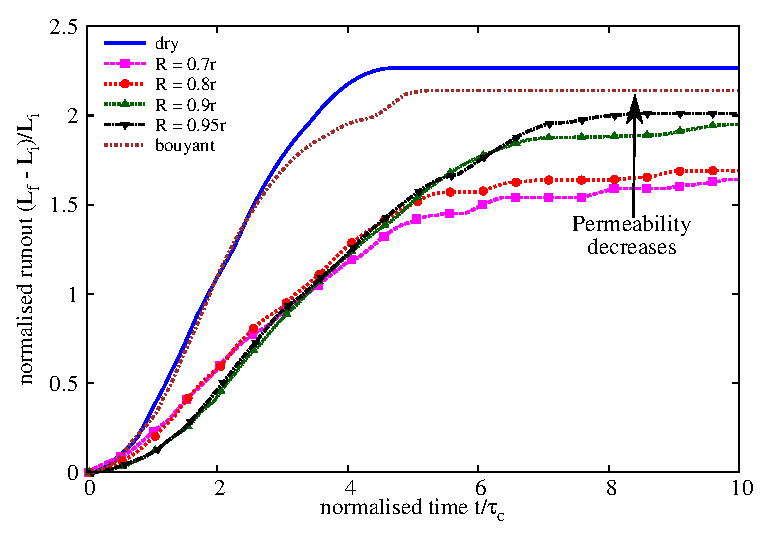
\includegraphics[width=0.9\textwidth]{Runout_a08_dense}
\caption{Effect of permeability on the evolution of run-out for a column 
collapse in fluid (a = 0.8)}
\label{fig:Runout_a08_dense}
\end{figure}

At a high permeability (r = 0.7 R), the evolution of run-out at the initial 
stage is quicker, which means that the negative pore-pressure that is developed 
during the shearing along the fracture surface is dissipated faster. Even 
though the negative pore-pressure is dissipated, due to 
the development of negative pore-pressure the evolution of run-out in fluid is 
slower than its dry counterpart. The rate of dissipation decreases with 
decrease in the permeability. This can be observed by a flatter slope in the 
run-out evolution with decrease in permeability.~\Cref{fig:PWP_ini_dense} shows 
the distribution of pore-pressure in high and low permeable granular media. At 
the same time $ t = \tau_c$, the highly permeable (r = 0.7 R) granular column 
shows smaller 
negative pore-pressure in comparison to large negative pore-pressures observed 
in the shearing zone of a low permeable column (r = 0.9 R). This shows that not 
only does it take longer for the pore-pressure to dissipate with a decrease 
in permeability, but also results in almost twice the negative pore-pressure 
than what is observed in the high permeable case 
(\cref{fig:r095_PWP_ini_dense}).

\begin{figure}
\centering
\begin{subfigure}[t]{0.975\textwidth}
	\centering
    \includegraphics[width=\textwidth]{a08/r07_PWP_ini_dense}
    \caption{High permeability (r = 0.7 R)}
    \label{fig:r07_PWP_ini_dense}
\end{subfigure} \\
\begin{subfigure}[t]{0.975\textwidth}
	\centering
    \includegraphics[width=\textwidth]{a08/r095_PWP_ini_dense}
    \caption{Low permeability (r = 0.95 R)}
    \label{fig:r095_PWP_ini_dense}
\end{subfigure}
\caption{Effect of permeability on the excess pore water pressure distribution 
for a granular column collapse in fluid (a = 0.8 \& dense packing) at $t = 
\tau_c$}
\label{fig:PWP_ini_dense}
\end{figure}

Although the low permeable granular columns require a longer duration for the 
run-out to evolve, the final run-out distance is found to be much longer than 
the high permeable condition.~\Cref{fig:PE_a08_dense} shows that the potential 
energy available for the flow of a low permeable column is 20\% smaller than 
the collapse of a high permeable granular column. The kinetic energy evolution 
(\cref{fig:a08_dense_energy}) shows that the low permeable column has a 
wider peak kinetic energy distribution in comparison to a sharp peak observed 
in the high permeable condition. This indicates the influence of lubrication, 
i.e., 
hydroplaning of the granular flow in low permeable conditions. The evolution of 
the horizontal kinetic energy with time reveals that the peak kinetic energy is 
sustained longer as the permeability of the granular material decreases 
(\cref{fig:KExy_a08_dense}). Although, the peak kinetic energy is smaller 
in the low permeability case, the hydroplaning of the flowing granular mass 
results in a longer run-out distance. A high positive pore-pressure is observed 
at the base of the granular flow in low permeability condition 
(\cref{fig:r095_PWP_flow_dense}) indicating the occurrence of hydroplaning. The 
evolution of local packing density shows a drop in the packing density at low 
permeability (\cref{fig:Packing_Density_a08_dense}). This drop in the value 
of packing density between $t = 2\tau_c$ and $t=3\tau_c$ corroborates with the 
duration of hydroplaning during which a large amount of water in entrained at 
the flow front.  

\begin{figure}
	\centering
    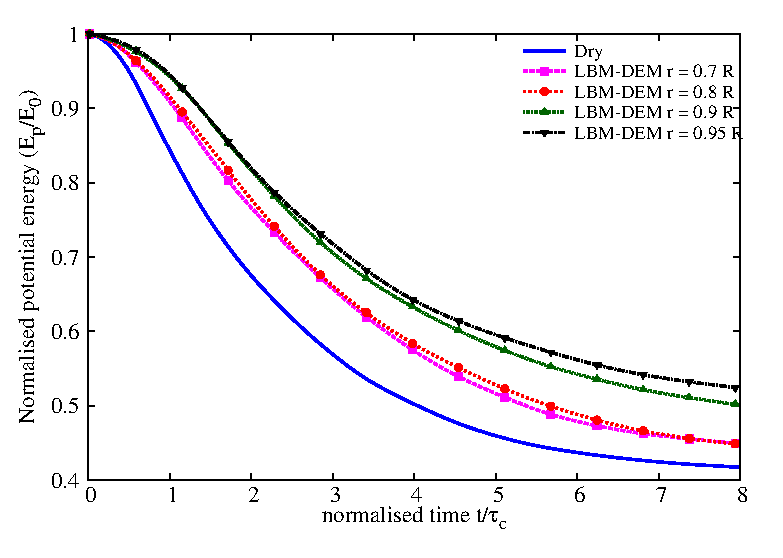
\includegraphics[width=0.7\textwidth]{PE_a08_dense}
    \caption{Effect of permeability on the evolution of the potential energy 
    with time for a granular column collapse in fluid (a = 0.8)}
    \label{fig:PE_a08_dense}
\end{figure}

\begin{figure}
\centering
\makebox[\linewidth][c]{
\begin{subfigure}[t]{0.8\textwidth}
	\centering
    \includegraphics[width=\textwidth]{KE_a08_dense}
    \caption{Evolution of the total kinetic energy}
    \label{fig:KE_a08_dense}
\end{subfigure}
}\\
\makebox[\linewidth][c]{
\begin{subfigure}[t]{0.95\textwidth}
	\centering
    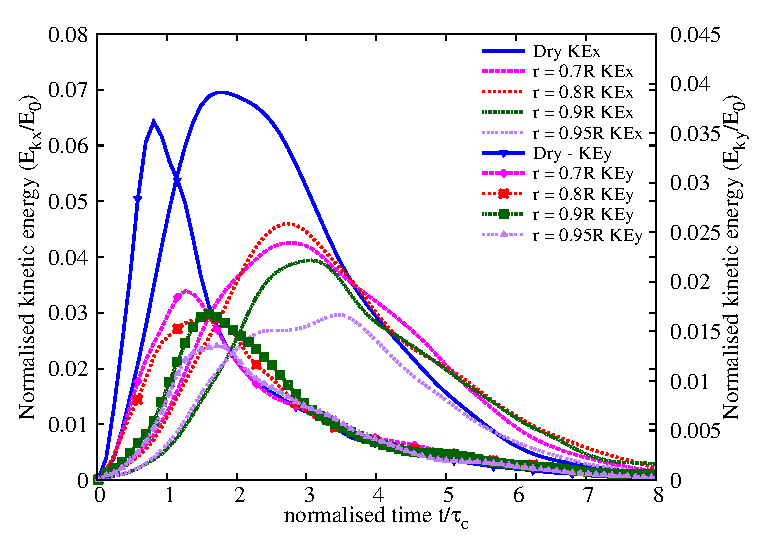
\includegraphics[width=\textwidth]{KExy_a08_dense}
    \caption{Evolution of horizontal and vertical kinetic energies}
    \label{fig:KExy_a08_dense}
\end{subfigure}
}
\caption{Effect of permeability on the evolution of kinetic energies with time 
for a granular column collapse in fluid (a = 0.8)}
\label{fig:a08_dense_energy}
\end{figure}


\begin{figure}
\centering
\begin{subfigure}[t]{0.975\textwidth}
	\centering
    \includegraphics[width=\textwidth]{a08/r07_PWP_flow_dense}
    \caption{High permeability (r = 0.7 R)}
    \label{fig:r07_PWP_flow_dense}
\end{subfigure}
\\
\begin{subfigure}[t]{0.975\textwidth}
	\centering
    \includegraphics[width=\textwidth]{a08/r095_PWP_flow_dense}
    \caption{Low permeability (r = 0.95 R)}
    \label{fig:r095_PWP_flow_dense}
\end{subfigure}
\caption{Effect of permeability on the excess pore water pressure distribution 
for a granular column collapse in fluid (a = 0.8 \& dense packing) at $t = 
2\tau_c$}
\label{fig:PWP_flow_dense}
\end{figure}

\begin{figure}
	\centering
    \includegraphics[width=0.8\textwidth]{Packing_Density_a08_dense}
    \caption{Effect of permeability on the evolution of packing density for a 
    granular column collapse in fluid (a = 0.8 \& dense initial packing)}
    \label{fig:Packing_Density_a08_dense}
\end{figure}

High permeable granular column shows lower water entrainment, which indicates 
that for highly permeable flows the drag force acting on the soil grains 
predominates over the lubrication effect on the run-out behaviour. In both the 
low and high permeable granular flows, the granular material consolidates at 
the final stage of the flow. This can be observed by the increase in the 
packing density at the final stage due to settlement of grains and expulsion of 
entrained water. The final deposit profile for both low and high permeability 
conditions are shown in~\cref{fig:a08_dense_snapshots}. The high permeable 
collapse show a more parabolic (convex) deposit profile in contrast to the more 
concave profile observed in the low permeability condition. The observation of 
hydroplaning in the low permeable condition may be due to the difference in the 
distribution of granular mass at the flow front. Instigation of hydroplaning is 
controlled by the balance of gravity and inertia forces at the debris front and 
is suitably characterized by the densimetric Froude's number:
%
\begin{equation}
Fr_d = \frac{U}{\sqrt{(\frac{\rho_d}{\rho_w}-1)gH\cos\theta}}
\end{equation}
where $U$ is the average velocity of sliding mass, $\rho_p$ and $\rho_w$ are 
the densities of soil and water, respectively, \textit{H} is the thickness of 
the sliding mass, \textit{g} is acceleration due to gravity and $\theta$ 
represents the slope angle.~\citet{Harbitz2003} observed 
hydroplaning above a critical value of densimetric Froude's number of 0.4. A 
Froude's $Fr_d$ value of 0.427 is observed for the low permeable flow (r = 0.95 
R), which indicates the occurrence of hydroplaning. Whereas, a $Fr_d = 0.273$ 
is observed for the high permeable granular flow indicating absence of 
hydroplaning, the low 
permeable collapse is predominated by the viscous drag force resulting in a 
parabolic profile and shorter run-out distance. 
\begin{figure}
\makebox[\linewidth][c]{
\begin{subfigure}[b]{0.85\textwidth}
	\centering
    \includegraphics[width=0.95\textwidth]{a08/a08r07_dense}
    \caption{High permeability (r = 0.7 R)}
    \label{fig:a08r07_dense}
\end{subfigure}
}\\
\makebox[\linewidth][c]{
\begin{subfigure}[b]{0.85\textwidth}
	\centering
    \includegraphics[width=0.95\textwidth]{a08/a08r095_dense}
    \caption{Low permeability (r = 0.95 R)}
    \label{fig:a08r095_dense}
\end{subfigure}
}
\caption{Effect of permeability on the deposit morphology of a granular column 
collapse in fluid (a = 0.8)}
\label{fig:a08_dense_snapshots}
\end{figure}

The normalised final run-out distance as a function of the initial aspect ratio 
of the column is presented in~\cref{fig:runout_fluid_dry}. For all aspect 
ratios, the dry condition yields the longest run-out distance. For a given 
aspect ratio, the dry collapse acquires the highest peak kinetic energy due to 
the lack of viscous dissipation during vertical collapse. This extra kinetic 
energy is high enough to propel the heap, in spite of a high frictional 
dissipation, over a distance that is longer than the run-out distance in 
the fluid regime. In the submerged condition, for the same aspect ratio, 
the kinetic energy available for spreading is lower and the dissipation 
due to viscous drag is higher, thus leading to a much shorter run-out
distance. 

For short columns, with decrease in permeability the run-out distance 
increases, however, the run-out distance is not higher than the dry condition. 
At higher aspect ratios, decrease in permeability from r = 0.8 R to r = 0.9 R 
does not have a significant influence on the run-out behaviour. This can be 
attributed to the turbulent nature of the granular flows for tall 
columns. The run-out behaviour is a result of transformation of (part of) the 
initial potential energy to the peak kinetic energy, which in turn controls the 
subsequent run-out along the plane. The run-out distance is plotted as a 
function of the normalised peak kinetic energy 
in~\cref{fig:runout_fluid_dry_energy}. For the same aspect ratio, the peak 
kinetic energy is higher in the case of dry column. This represents grain 
inertial regime in dry granular collapse, which indicates that a part of the 
potential energy, in the presence of the fluid, is dissipated during the 
vertical collapse due to viscous friction. In all regimes, the 
run-out distance increases as a power law $L_f \propto KE_{max}^\gamma$. For 
the same value of peak kinetic energy, the run-out distance in fluid is longer 
than the dry column collapse. Also, with decrease in 
permeability the run-out distance increases for the same peak kinetic energy. 
\begin{figure}[tbhp]
	\centering
	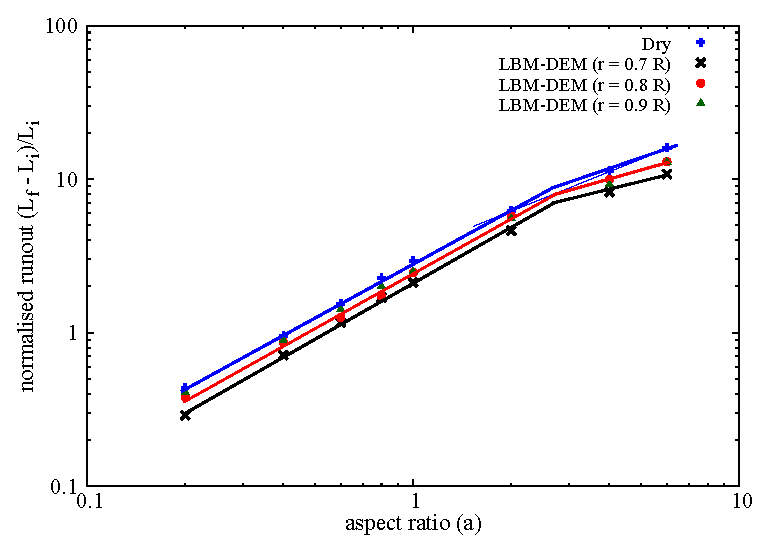
\includegraphics[width=0.95\textwidth]{runout_fluid_dry}
	\caption{Normalised final run-out distance for columns with different 
	initial aspect ratios. Comparison of dry and submerged granular column 
	collapse for different hydrodynamic radius (0.7 R, 0.8 R and 0.9 R).}
	\label{fig:runout_fluid_dry}
\end{figure} 

\begin{landscape}
\begin{figure}
	\centering
	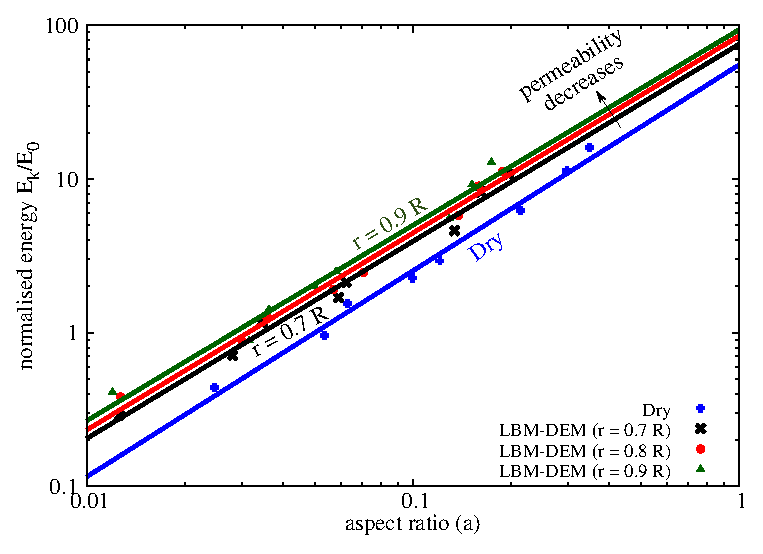
\includegraphics[height=0.9\textheight]{runout_fluid_dry_energy}
	\caption[Normalised final run-out distance for columns as a function of 
		peak kinetic energy in dry and submerged conditions]{Normalised final 
		run-out distance for columns as a function of 
	peak kinetic energy. Comparison of dry and submerged granular column 
	collapse for different hydrodynamic radius (0.7 R, 0.8 R and 0.9 R).}
	\label{fig:runout_fluid_dry_energy}
\end{figure}
\end{landscape}

%	\caption{Normalised final run-out distance as a function of initial aspect 
%	ratio and the peak kinetic energy.}
%	\label{fig:runout_fluid}
%\end{figure}


\subsection{Effect of initial packing density}

\citet{Rondon2011} observed that the loose packings flow rapidly on a time
scale proportional to the initial height and results in longer run-out distance 
in comparison to the dense packing. Hydroplaning occurs above a critical 
Froude's number of 0.4. The Froude's number is inversely related to the 
thickness of the flow and its density. Hence, for the same thickness of flow, a 
loose granular column will experience more hydroplaning than a dense granular 
flow. This effect might result in longer run-out behaviour in fluid than the 
dry condition for the same initial aspect ratio. The initial packing density 
and the permeability of a 2D granular column, with an aspect ratio of 0.8, are 
varied to understand their influence on the run-out behaviour. The run-out 
behaviour of the dense case (83\% packing density), discussed in the previous 
section, is compared with a loose granular column (79\% packing fraction). The 
permeability is varied by changing the hydrodynamic radius from 0.7 R to 0.95 
R. 

The normalised run-out evolution with time for a loose initial packing (79\% 
packing fraction) with different hydrodynamic radii 0.7 R, 0.8 R, 0.9 and 0.95 
R are presented in~\cref{fig:Runout_a08_loose}. The run-out evolution of dry 
and a column with grains in suspension with an 
initial aspect ratio of 0.8 are also presented to understand the influence of 
hydrodynamic forces on the flow kinematics. Similar to the dense granular 
column, the run-out distance increases with increase in the hydrodynamic radius 
(i.e., decrease in permeability). At low permeabilities (r = 0.9 and 0.95 R), 
the run-out distance is longer than the dry condition. This shows that the 
lubrication effect in low permeability condition overcomes the influence of 
the drag force and the development of large negative pore-pressure resulting in 
a longer run-out distance. Although suspended granular masses experience high 
drag 
force and turbulent effects, the run-out evolves almost at the same rate in 
comparison with granular columns with high permeability. This shows the effect 
of permeability on the dissipation rate of negative pore-pressure developed 
during the initial stage of collapse.

\begin{figure}
\centering
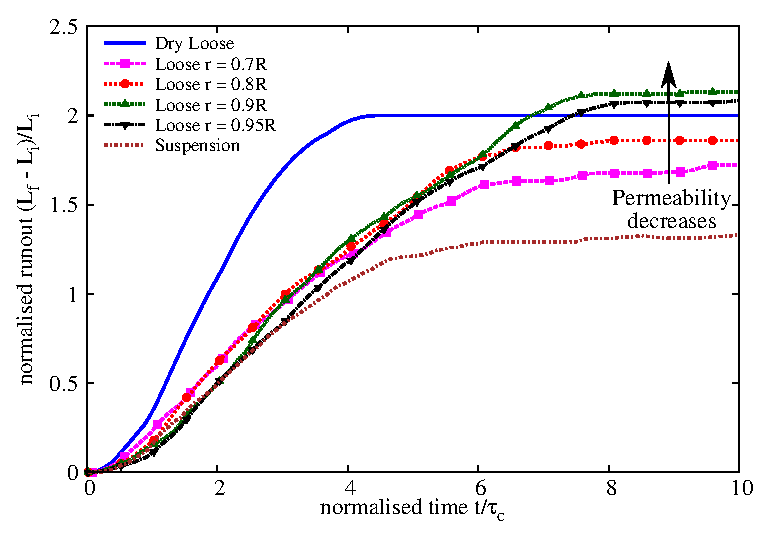
\includegraphics[width=0.9\textwidth]{Runout_a08_loose}
\caption{Effect of permeability on the evolution of run-out for a column 
collapse in fluid (a = 0.8 \& loose packing)}
\label{fig:Runout_a08_loose}
\end{figure}

\Cref{fig:Loose_PWP_ini} shows the development of negative pore-pressure in low 
permeability (r = 0.95 R) and dissipation of negative pore-pressure in high 
permeability (r = 0.7 R) at the same time $ t = \tau_c$. This difference in the 
quantity and the rate of dissipation of negative pore-pressure results in 
a difference in the rate of flow evolution. A low permeable column requires a 
longer 
duration to evolve. As the flow progresses, the low permeability of 
the granular column causes hydroplaning to occur at the base of the column 
resulting in longer run-out distance (\cref{fig:Loose_PWP_flow}).
\begin{figure}
\centering
\makebox[\linewidth][c]{
\begin{subfigure}[t]{0.975\textwidth}
	\centering
    \includegraphics[width=\textwidth]{a08/Loose_r07_PWP_ini}
    \caption{High permeability (r = 0.7 R)}
    \label{fig:Loose_r07_PWP_ini}
\end{subfigure}
}\\
\makebox[\linewidth][c]{
\begin{subfigure}[t]{0.975\textwidth}
	\centering
    \includegraphics[width=\textwidth]{a08/Loose_r095_PWP_ini}
    \caption{Low permeability (r = 0.95 R)}
    \label{fig:Loose_r095_PWP_ini}
\end{subfigure}
}
\caption{Effect of permeability on the excess pore water pressure distribution 
for a granular column collapse in fluid (a = 0.8 \& loose packing) at $t = 
\tau_c$}
\label{fig:Loose_PWP_ini}
\end{figure}

\begin{figure}
\centering
\makebox[\linewidth][c]{
\begin{subfigure}[t]{0.975\textwidth}
	\centering
    \includegraphics[width=\textwidth]{a08/Loose_r07_PWP_flow}
    \caption{High permeability (r = 0.7 R)}
    \label{fig:Loose_r07_PWP_flow}
\end{subfigure}
}\\
\makebox[\linewidth][c]{
\begin{subfigure}[t]{0.975\textwidth}
	\centering
    \includegraphics[width=\textwidth]{a08/Loose_r095_PWP_flow}
    \caption{Low permeability (r = 0.95 R)}
    \label{fig:Loose_r095_PWP_flow}
\end{subfigure}
}
\caption{Effect of permeability on the excess pore water pressure distribution 
for a granular column collapse in fluid (a = 0.8 \& loose packing) at $t = 
2\tau_c$}
\label{fig:Loose_PWP_flow}
\end{figure}

The evolution of the potential energy with time reveals that at a very low 
permeability (r = 0.95 R), the initial potential energy mobilised is smaller 
than at r = 0.9 R. Also with decrease in permeability, the time required to 
dissipate the negative pore-pressure increases. This results in a shorter 
run-out distance in the case of r = 0.95 R to that of r = 0.9 R. As the 
quantity of material destabilised is small, the flow is thinner and thus has a 
high Froude's number. However, the peak horizontal kinetic velocity observed in 
the case of r = 0.9 R is higher than r = 0.95 R 
(\cref{fig:KExy_a08_loose}).  A Froude's number of 0.59 for r = 0.9 R is 
observed in contrast to 0.46 for r = 0.95 R. Both values of hydrodynamic radii 
result in a Froude's number that indicates occurrence of hydroplaning. However, 
the difference in the amount of material destabilised for r = 0.95 R and the 
decreased effect of hydroplaning results in a shorter run-out distance for r = 
0.95 R in comparison to r = 0.9 R. 


As the column collapses, water is entrained at the flow front. This can 
observed by the decrease in the packing fraction during $t = 1\tau_c$ and $t = 
3\tau_c$. As the flow progresses, the entrained water is expelled and the soil 
grains consolidate to reach a critical packing density at the end of the flow 
(\cref{fig:Packing_Density_a08_loose}). The permeability (hydrodynamic 
radius) plays a crucial role in the rate of dissipation of the entrained water. 
As the permeability decreases, the water entrained at the flow front takes 
longer time to be dissipated resulting in lubrication of the flow at low 
permeabilities. This lubrication effect results in an increase in the run-out 
distance for columns with low permeabilities.

\begin{figure}
	\centering
    \includegraphics[width=0.8\textwidth]{PE_a08_loose}
    \caption{Effect of permeability on the evolution of the potential energy 
    with time for a granular column collapse in fluid (a = 0.8 \& loose 
    packing)}
    \label{fig:PE_a08_loose}
\end{figure}


\begin{figure}
	\centering
    \includegraphics[width=0.8\textwidth]{Packing_Density_a08_loose}
    \caption{Effect of permeability on the evolution of packing density for a 
    granular column collapse in fluid (a = 0.8 \& loose initial packing)}
    \label{fig:Packing_Density_a08_loose}
\end{figure}

\begin{figure}
\centering
\makebox[\linewidth][c]{
\begin{subfigure}[t]{0.8\textwidth}
	\centering
    \includegraphics[width=\textwidth]{KE_a08_loose}
    \caption{Evolution of the total kinetic energy}
    \label{fig:KE_a08_loose}
\end{subfigure}
}\\
\makebox[\linewidth][c]{
\begin{subfigure}[t]{0.95\textwidth}
	\centering
    \includegraphics[width=\textwidth]{KExy_a08_loose}
    \caption{Evolution of horizontal and vertical kinetic energies}
    \label{fig:KExy_a08_loose}
\end{subfigure}
}
\caption{Effect of permeability on the evolution of kinetic energies with time 
for a granular column collapse in fluid (a = 0.8 \& loose packing)}
\label{fig:a08_loose_energy}
\end{figure}

The evolution of grain trajectories with time are presented 
in~\cref{fig:Loose_a08_permeability} for low (r = 0.95 R) and high (r = 0.9 R)
permeability conditions. It can be observed that a high 
permeability column shows a parabolic (convex) final profile in contrast to the 
more concave profile observed in low permeability condition. This difference in 
the flow thickness results in a higher value of Froude's number and the 
occurrence of hydroplaning in the low permeability condition. Due to the high 
permeability, the water entrained at the flow front is dissipated quicker and 
thus no lubrication effect is observed. A Froude's number of 0.272 (no 
hydroplaning) is observed for the high permeability condition (r = 0.7 R). This 
shows that the drag force predominates at high permeability, while the low 
permeability condition is characterised by hydroplaning and lubrication.

\Cref{fig:effective_stress_a08} shows the normalised pressure at the 
base for the low and high permeability flows at $ t = 2\tau_c$. The normalised 
effective stress plotted is obtained as the average over 5 time steps at 
$2\tau_c$. The effective stress at the base is normalised to the effective 
stress of a static granular column before the collapse. A value of 1 indicates 
that 
the effective stress hasn't changed, which can be observed in the static region 
of 
the granular column. It can be observed that the normalised effective stress is 
significantly higher for the high permeability condition at the flow front in 
comparison to the almost non-existence of effective stress in the low 
permeability condition. The observation of trivial effective stress at the flow 
front 
corroborates the lubrication effect observed at low permeability conditions.

\begin{figure}
\centering
\makebox[\linewidth][c]{
\begin{subfigure}[t]{0.975\textwidth}
	\centering
    \includegraphics[width=\textwidth]{a08/LBM_MD_loose_a08_r07_pt}
    \caption{High permeability (r = 0.7 R)}
    \label{fig:LBM_MD_loose_a08_r07_pt}
\end{subfigure}
}\\
\makebox[\linewidth][c]{
\begin{subfigure}[t]{0.975\textwidth}
	\centering
    \includegraphics[width=\textwidth]{a08/LBM_MD_a08_Loose_r09}
    \caption{Low permeability (r = 0.95 R)}
    \label{fig:LBM_MD_a08_Loose_r09}
\end{subfigure}
}
\caption{Particle tracking of the deposit morphology
for a granular column collapse in fluid (a = 0.8 \& loose packing), influence 
of permeability}
\label{fig:Loose_a08_permeability}
\end{figure}

\begin{figure}
\centering
\includegraphics[width=0.97\columnwidth]{a08/effective_stress_a08}
\caption{Effect of permeability on the normalised effective stress for loose 
initial packing at $t = 2\tau_c$}
\label{fig:effective_stress_a08}
\end{figure}

\Cref{fig:Dense_Loose_PT} shows the grain trajectories of a dense and a loose 
initial packing for a hydrodynamic radius (r = 0.95 R). It can be observed that 
the dense initial packing results in a lot of turbulent behaviour at the flow 
surface in contrast to the more plug like flow observed in the loose condition. 
The thickness of the deposit in both dense and loose condition is almost the 
same, however the density of the flow results in a Froude's number of 0.46 and
0.429 for loose and dense conditions, respectively. The low initial density 
results in more hydroplaning in the loose condition. The effect of water 
entrainment at the flow front between dense and loose condition can be seen 
in~\cref{fig:Dense_Loose_voro}. Comparing the packing density 
(\cref{fig:Packing_Density_a08_dense,fig:Packing_Density_a08_loose}) 
reveals almost the same amount of water entrainment in both dense and loose 
conditions. Hence, it is the density of the flowing granular mass that controls 
the influence of hydroplaning for a given hydrodynamic radius and initial 
aspect ratio. A loosely packed granular column with low permeability entrains 
more water at the flow front, resulting in a hydroplaning effect that overcomes 
the influence of viscous drag forces and thereby yields a higher run-out 
distance than the dry condition.

\citet{Rondon2011} also observed that the collapse of a granular column in a 
viscous fluid is mainly controlled by the initial volume fraction and not by 
the aspect ratio of the column. The role of the initial volume fraction 
observed explains the pore pressure feedback mechanism proposed 
by~\citep{Schaeffer2008,Iverson2000} in the context of landslides. The 
compaction or dilation of grains can cause additional stress in the grains 
which can stabilise or destabilise the soil. The flow is thus controlled by the 
coupling between the dilatancy of the granular layer and the development of 
pore pressure in the fluid phase~\citep{Pailha2008}. The dense column needs to 
dilate in order to flow. When it starts to fall, liquid is then sucked into the 
column, which is then stabilized by the additional viscous 
drag~\citep{Rondon2011,Topin2012}. By opposition the loose column when 
it starts flowing expands and ejects liquid, leading to a partial fluidisation 
of the material.

\begin{figure}
\centering
\makebox[\linewidth][c]{
\begin{subfigure}[t]{0.975\textwidth}
	\centering
    \includegraphics[width=\textwidth]{a08/PT_Dense_R095}
    \caption{Dense initial packing (83\%)}
    \label{fig:PT_Dense_R095}
\end{subfigure}
}\\
\makebox[\linewidth][c]{
\begin{subfigure}[t]{0.975\textwidth}
	\centering
    \includegraphics[width=\textwidth]{a08/PT_Loose_R095}
    \caption{Loose initial packing (79\%)}
    \label{fig:PT_Loose_R095}
\end{subfigure}
}
\caption[Effect of initial density on the deposit morphology
for a granular column collapse in fluid (a = 0.8).]{Effect of initial density 
on the deposit morphology
for a granular column collapse in fluid (a = 0.8). Dense vs loose initial 
packing fraction (r = 0.95 R). Darker means dense packing, white indicates 
loose 
packing density.}
\label{fig:Dense_Loose_PT}
\end{figure}


\begin{figure}
\centering
\makebox[\linewidth][c]{
\begin{subfigure}[t]{0.975\textwidth}
	\centering
    \includegraphics[width=\textwidth]{a08/Dense_a08_voro_tc}
    \caption{Dense initial packing (83\%)}
    \label{fig:Dense_a08_voro_tc}
\end{subfigure}
}\\
\makebox[\linewidth][c]{
\begin{subfigure}[t]{0.975\textwidth}
	\centering
    \includegraphics[width=\textwidth]{a08/Loose_a08_voro_tc}
    \caption{Loose initial packing (79\%)}
    \label{fig:Loose_a08_voro_tc}
\end{subfigure}
}
\caption{Evolution of packing fraction at $t = \tau_c$ for dense and loose 
initial packing fraction.}
\label{fig:Dense_Loose_voro}
\end{figure}

\clearpage


\section{Submarine granular flows down incline plane}

Slope failure is a problem of high practical importance for both civil 
engineering structures and natural hazards management. Catastrophic events such 
as landslides, debris flows, rock avalanches or reservoir embankment failures 
exemplify the potential consequences of a soil gravitational instability. One 
of the most critical situations concerns a submerged sandy slope as pore 
pressure changes, seepage or earthquakes can cause significant damages to 
off-shore structures and may generate a tsunami.

The influence of slope angle on the effect of permeability and the initial 
packing density on the run-out behaviour are studied. In this study, a 2D 
poly-disperse system ($d_{max}/d_{min} = 2$) of circular discs forming a 
granular column in fluid is used to understand 
the behaviour of granular flows down inclined planes (\Cref{fig:LBM_Scheme_geometry}). 
The soil column is modelled using $\sim 1000$ to $2000$ discs of density 
\SI{2650}{\kg\per\cubic\meter} and a contact friction angle of 
\SI{26}{\degree}. The collapse of the granular column is simulated inside a 
fluid with a density of \SI{1000}{\kg\per\cubic\meter} and a kinematic 
viscosity of \SI{1e-6}{\square\meter\per\second}. A granular column with 
an 
initial aspect ratio \textit{a} of 0.8 is used. A hydrodynamic radius r = 0.9 R 
is adopted during the LBM computations. Dry analyses are also performed to 
study the effect of hydrodynamic forces on the run-out distance. The 
numerical configuration used in this study is shown in~\cref{fig:geometry}. The 
slope angle $\theta$ is varied as \SI{0}{\degree}, \SI{2.5}{\degree}, 
\SI{5}{\degree}, and \SI{7.5}{\degree}. The effect of initial packing density 
is studied using a 
dense packing (83\% packing fraction) and a loose packing (79\% packing 
fraction) of granular columns that collapse on to an inclined plane at 
different slope angles. The influence of permeability (with hydrodynamic radius 
varied as 0.7, 0.75, 0.8, 0.85 and 0.9 R) on the run-out behaviour of collapse 
of granular columns with initial packing density of 83\% and 79 \% on to an 
inclined plane with a slope angle of 5\si{\degree} is also analysed. 


\subsection{Effect of initial density}
The morphology of granular deposits in fluid is shown to be mainly 
controlled by the initial volume fraction of the granular mass and not by the 
aspect ratio of the column~\citep{Rondon2011,Pailha2008}. In order to 
understand the influence of the initial packing density on the run-out 
behaviour, a dense sand column (initial packing density, $\Phi=83\%$) and a 
loose sand column ($\Phi=79\%$) are considered. The granular columns collapse 
and flow down slopes of varying inclinations (\SI{2.5}{\degree}, 
\SI{5}{\degree} and \SI{7.5}{\degree}). The run-out behaviour is compared with 
the collapse of a granular column in fluid on a horizontal surface. For all 
slope angles, the flow kinematics in the submerged condition is compared with 
its dry counterpart to understand the influence of lubrication and viscous 
drag. A hydrodynamic radius of r = 0.9 R is adopted in all cases, because low 
permeability conditions result in longer run-out distance as observed in the 
previous section.


The evolution of run-out for a dense sand column with time in dry and submerged 
conditions for varying slope inclinations are presented 
in~\cref{fig:run_dense}. For all slope angles, the run-out distances in the dry 
condition are longer than those observed in the submerged condition. Similar to 
the case of collapse on a horizontal plane, the dense granular columns 
experience drag forces that have a significant influence than the lubrication 
effect. The difference in the run-out between the dry and the submerged 
condition 
decreases with increase in the slope angle. At a slope angle of 5\si{\degree} 
the 
difference in the run-out between 
the dry and the submerged condition is the smallest. This is due to significant 
hydroplaning of a thin flowing layer, the occurrence of hydroplaning can be 
observed by a sustained peak kinetic energy (\cref{fig:KE_dense}). At 
higher slope angles (> 5\si{\degree}), the drag force predominates over the 
lubrication effect and results in shorter run-out distance. 
\begin{figure}
\centering
\begin{subfigure}[t]{0.95\textwidth}
\centering
\includegraphics[width=0.95\columnwidth]{Runout_dense_slope}
\caption{Evolution of run-out with time (dense)}
\label{fig:run_dense}
\end{subfigure}\\
\begin{subfigure}[t]{0.95\textwidth}
\centering
\includegraphics[width=0.95\columnwidth]{KE_dense_slope}
\caption{Evolution of kinetic energy with time (dense case)}
\label{fig:KE_dense}
\end{subfigure}
\caption{Evolution of run-out and kinetic energy with time (dense)}
\label{fig:run_KE_dense}
\end{figure}

Similar to the case of collapse on a horizontal surface, the dense granular 
columns 
in fluid require a longer time to collapse and flow, due to the development of 
large negative pore-pressures. Large negative pore-pressures are developed as 
the 
dense granular material dilates due to shearing along the fracture surface in 
the initial phase of the flow. The snapshots of the dense granular column 
collapse down slopes of varying inclinations at the time 
($t=\tau_{c}=3\sqrt{H/g}$), are shown in~\cref{fig:slope_dense}.

It can be seen that the viscous drag on the dense column tends to predominate 
over the influence of hydroplaning on the run-out behaviour. This influence can 
be observed in the smaller peak kinetic energy for submerged granular in 
comparison to the dry condition (\Cref{fig:KE_dense}). With increase in 
the slope angle, the volume of material that dilates increases. This results in 
large negative pore-pressures and more viscous drag on the granular material. 
Hence, the difference in the run-out between the dry and the submerged 
conditions, for a dense granular assembly, increases with increase in the slope 
angle above an inclination of 5\si{\degree}.


\begin{figure}
\makebox[\linewidth][c]{
\begin{subfigure}[b]{0.95\textwidth}
	\centering
    \includegraphics[width=0.95\textwidth]{dense_slope/dense_slope25r09}
    \caption{Slope 2.5}
    \label{fig:ds2.5}
\end{subfigure}
}\\

\makebox[\linewidth][c]{
\begin{subfigure}[b]{0.95\textwidth}
	\centering
    \includegraphics[width=0.95\textwidth]{dense_slope/dense_slope5r09}
    \caption{Slope 5.0}
    \label{fig:ds5.0}
\end{subfigure}
}\\

\makebox[\linewidth][c]{
\begin{subfigure}[b]{0.95\textwidth}
	\centering
    \includegraphics[width=0.95\textwidth]{dense_slope/dense_slope75r09}
    \caption{Slope 7.5}
    \label{fig:ds7.5}
\end{subfigure}
}
\caption{Flow morphology at $t = 3 \tau_c$ for different slope angles (dense)}
\label{fig:slope_dense}
\end{figure}

In contrast to the dense granular columns, the loose granular columns (packing 
fraction of 79\%) show longer run-out distance in immersed conditions 
(\Cref{fig:run_loose}). The run-out distance in fluid increases with 
increase in the slope angle in comparison to the dry cases. The loose granular 
flow tends to entrain more water at the base of the flow 
front, creating a lubricating surface, which results in a longer run-out 
distance (\Cref{fig:slope_loose}). For the same thickness of the flow, 
the loose granular flow has smaller density and hence a higher Froude's number 
than the dense flow resulting in a higher probability of hydroplaning. The 
hydroplaning effect causes an increase in the flow velocity for the loose 
granular material in comparison with the dense condition 
(\Cref{fig:KE_loose}).

\begin{figure}
\centering
\begin{subfigure}[b]{0.95\textwidth}
\centering
\includegraphics[width=0.97\columnwidth]{Runout_loose_slope}
\caption{Evolution of run-out with time (loose)}
\label{fig:run_loose}
\end{subfigure} \\
\begin{subfigure}[b]{0.95\textwidth}
\centering
\includegraphics[width=0.97\columnwidth]{KE_loose_slope}
\caption{Evolution of kinetic energy with time (loose)}
\label{fig:KE_loose}
\end{subfigure}
\caption[Evolution of run-out and kinetic energy with time (loose) for 
different slope angles]{Evolution of run-out and kinetic energy with time 
(loose)}
\label{fig:KE_run_loose}
\end{figure}

The snapshots at $t = 3\tau_c$ of a loose granular column (a = 0.8) collapse 
down slopes inclined at an angle of 2.5\si{\degree}, 5\si{\degree} and 
7.5\si{\degree} are presented in~\cref{fig:slope_loose}. In contrast to dense 
granular flows, a plug-like flow can be observed. Due to the low permeability, 
the 
water entrapped in the flow front results in a drop in the density of the 
flowing mass thus enabling hydroplaning. The turbulence effect observed on the 
surface of the dense granular flow is absent in the loose granular collapse. 
This, along with the lubrication effect, results in a longer run-out distance 
in the submerged condition for a loose granular column than the dry collapse. 

\begin{figure}
\makebox[\linewidth][c]{
\begin{subfigure}[b]{0.95\textwidth}
	\centering
    \includegraphics[width=0.95\textwidth]{loose_slope/loose_slope25r09}
    \caption{Slope 2.5}
    \label{fig:ls2.5}
\end{subfigure}
}\\

\makebox[\linewidth][c]{
\begin{subfigure}[b]{0.95\textwidth}
	\centering
    \includegraphics[width=0.95\textwidth]{loose_slope/loose_slope5r09}
    \caption{Slope 5.0}
    \label{fig:ls5.0}
\end{subfigure}
}\\

\makebox[\linewidth][c]{
\begin{subfigure}[b]{0.95\textwidth}
	\centering
    \includegraphics[width=0.95\textwidth]{loose_slope/loose_slope75r09}
    \caption{Slope 7.5}
    \label{fig:ls7.5}
\end{subfigure}
}
\caption{Flow morphology at time $t = 3\tau_c$ for different slope angles 
(loose)}
\label{fig:slope_loose}
\end{figure}


The evolution of packing density (\cref{fig:voro}) shows that, at the end 
of the flow, both the dense and the loose conditions reach similar packing 
density. 
This indicates that the dense granular column dilates more and is susceptible 
to higher viscous drag forces. Whereas in the loose condition, a positive 
pore-pressure is observed at the base of the flow, indicating entrainment of 
water at the base, i.e. lubrication and drop in the effective stress resulting 
in a longer run-out distance. The amount of water entrained in the loose 
granular 
column is higher than the dense condition, this can be observed by the low 
packing fraction observed between $2\tau_c$ and $5 \tau_c$. 

\begin{figure}
\centering
\includegraphics[width=0.97\columnwidth]{Voronoi_Slope_Dense_Loose}
\caption{Evolution of packing density with time for different slope angles}
\label{fig:voro}
\end{figure}

\Cref{fig:slope_runout_dense} shows the evolution of run-out with slope angle 
for an initially dense granular column. With increase in the slope angle, the 
run-out increases in both dry and submerged conditions. For all slope angles, 
the run-out in the dry condition is higher than the submerged conditions. As 
the slope angle increases, the drag force experienced by the dense granular 
column predominates over the lubrication effect on the run-out behaviour, this 
results in an increase in the difference between the dry and the submerged 
conditions with increase in the slope angle. Whereas with increase in slope 
angle, the loose granular column flows longer than the dry conditions. The 
longer run-out in the loose granular column collapse is due to hydroplaning 
experienced at the flow front as a result of entrainment of 
water.~\Cref{fig:slope_runout} shows that for a 
given initial aspect ratio and slope angle, the run-out distance in the loose 
granular collapse in fluid is higher than the dense condition. This observation 
in fluid is in contrast to the dry condition, where the dense granular column 
flows longer due to higher initial potential energy. The low permeability 
observed in the loose granular flow ensures that water entrained at the base of 
the flow front is retained resulting in sustained lubrication effect. Also, the 
low permeability ensures that the density of the flowing mass remains in a 
slurry state resulting in a longer duration of hydroplaning. These effects in 
the loose granular column with low permeability condition result in a longer 
run-out distance. 

\begin{figure}
	\centering
\begin{subfigure}[b]{0.95\textwidth}
	\centering
    \includegraphics[width=0.95\textwidth]{slope_runout_dense}
    \caption{Dense}
    \label{fig:slope_runout_dense}
\end{subfigure}\\
\begin{subfigure}[b]{0.95\textwidth}
	\centering
    \includegraphics[width=0.95\textwidth]{slope_runout_loose}
    \caption{Loose}
    \label{fig:slope_runout_loose}
\end{subfigure}
\caption{Comparison between dry and submerged granular column on the effect of 
slope angle on the run-out distance (Dense and Loose).}
\label{fig:slope_loose_dense}
\end{figure}


\begin{figure}
\centering
\includegraphics[width=0.97\columnwidth]{slope_runout}
\caption{Effect of slope angle on the run-out behaviour for different initial 
packing density.}
\label{fig:slope_runout}
\end{figure}

\clearpage
\subsection{Effect of permeability}

In order to understand the effect of permeability at a slope angle of 
\SI{5}{\degree}, the collapse of a granular column with an initial aspect ratio 
of 0.8 is simulated with different permeabilities. The hydrodynamic radius of 
a loosely packed granular column is varied from r = 0.7 R (high permeability), 
0.75 R, 0.8 R, 0.85 R to 0.9 R (low permeability). The run-out distance is 
found to increase with decrease in the permeability of the granular assembly 
(\Cref{fig:run5}). The run-out distance for high permeable conditions (r = 
0.7 R -- 0.8 R) are lower than their dry counterparts. Although, decrease in 
permeability resulted in an increase in the run-out distance, no significant 
change in the run-out behaviour is observed for a hydrodynamic radius of up to 
0.8 R.

With further decrease in permeability (r = 0.85 R and 0.9 R), the run-out 
distance in the fluid is longer than that observed in the dry 
condition. At a very low permeability (r = 0.9 R), the flowing granular mass
entrains more water at the base, which causes a reduction in the effective 
stress accompanied by a lubrication effect on the flowing granular media. This 
can be seen by a significant increase in the peak kinetic energy and the 
duration of the peak energy, in comparison to the dry and the highly permeable 
conditions (\Cref{fig:KE5}). However, the permeability of the granular 
column did not have an influence on the evolution of height during the flow. 
But, the dry granular column tends to collapse more than the immersed granular 
column due to lack of viscous dissipation (\Cref{fig:height5}).

\begin{figure}
\centering
\begin{subfigure}[b]{0.95\textwidth}
\centering
\includegraphics[width=0.95\columnwidth]{Runout_loose_5_slope}
\caption{Evolution of run-out with time}
\label{fig:run5}
\end{subfigure}\\
\begin{subfigure}[b]{0.95\textwidth}
\centering
\includegraphics[width=0.95\columnwidth]{Height_loose_5_slope}
\caption{Evolution of height with time}
\label{fig:height5}
\end{subfigure}
\caption{Evolution of run-out and height with time for different permeability 
(loose slope \SI{5}{\degree})}
\label{fig:height_run_5}
\end{figure}

\begin{figure}
\centering
\begin{subfigure}[b]{0.95\textwidth}
\includegraphics[width=0.95\columnwidth]{KE_loose_5_slope}
\caption{Evolution of kinetic energy with time}
\label{fig:KE5}
\end{subfigure} \\
\begin{subfigure}[b]{0.95\textwidth}
\centering
\includegraphics[width=0.95\columnwidth]{Voronoi_5}
\caption{Evolution of packing density with time}
\label{fig:voro5}
\end{subfigure}
\caption{Evolution of kinetic energy and packing density with time for 
different permeability (loose slope \SI{5}{\degree})}
\label{fig:voro_ke_5}
\end{figure}

\begin{figure}
\makebox[\linewidth][c]{
\begin{subfigure}[b]{0.95\textwidth}
	\centering
    \includegraphics[width=0.95\textwidth]{loose_slope/LBM_660_Slope5_r07}
    \caption{r = 0.7 R}
    \label{fig:LBM_660_Slope5_r07}
\end{subfigure}
}\\
\makebox[\linewidth][c]{
\begin{subfigure}[b]{0.95\textwidth}
	\centering
    \includegraphics[width=0.95\textwidth]{loose_slope/LBM_660_Slope5_r075}
    \caption{r = 0.75 R}
    \label{fig:LBM_660_Slope5_r075}
\end{subfigure}
} \\
\makebox[\linewidth][c]{
\begin{subfigure}[b]{0.95\textwidth}
	\centering
    \includegraphics[width=0.95\textwidth]{loose_slope/LBM_660_Slope5_r08}
    \caption{r = 0.8 R}
    \label{fig:LBM_660_Slope5_r08}
\end{subfigure}
}\\
\makebox[\linewidth][c]{
\begin{subfigure}[b]{0.95\textwidth}
	\centering
    \includegraphics[width=0.95\textwidth]{loose_slope/LBM_660_Slope5_r085}
    \caption{r = 0.85 R}
    \label{fig:LBM_660_Slope5_r085}
\end{subfigure}
}\\
\makebox[\linewidth][c]{
\begin{subfigure}[b]{0.95\textwidth}
	\centering
    \includegraphics[width=0.95\textwidth]{loose_slope/LBM_660_Slope5_r09}
    \caption{r = 0.9 R}
    \label{fig:LBM_660_Slope5_r09}
\end{subfigure}
}
\caption{Evolution of the flow front at $t = 3\tau_c$ for different 
permeabilities (loose slope 5\si{\degree}).}
\label{fig:slope_loose_5}
\end{figure}

Positive pore-pressure generation at the base of the flow is observed for low 
permeable conditions. Inspection of the local packing density showed 
entrainment of water at the base of the flow, which can also be observed by the 
steep decrease in the packing density (\Cref{fig:voro5}) for the very low 
permeability condition (r = 0.9 R). At the end of the flow ($t \ge 10 \times 
\tau_c$), the excess pore-pressure dissipates and the granular flows, 
irrespective of their permeability, reach almost the same packing density.


\Cref{fig:Perm_Runout_loose_dense} shows the effect of permeability on the 
run-out behaviour for a dense and a loose granular column collapse on a slope 
of 5\si{\degree} and 0\si{\degree}. In both cases, the run-out distance 
increases with increase in the hydrodynamic radius (decrease in permeability). 
However in the dense case, the run-out distance observed in the fluid is 
shorter than the dry condition. Whereas in the loose condition, the run-out 
distance increases significantly at low permeabilities and results in a longer 
run-out distance in the submerged condition in comparison to the dry granular 
collapse. The comparison of loose and dense collapse on a slope of 
0\si{\degree} and 5\si{\degree} shows that the initial packing density plays a 
significant role in the case of collapse on a horizontal plane, however at a 
slope of 5\si{\degree}, the run-out distance is unaffected by the initial 
packing density at high permeability conditions. This shows that at high 
permeabilities, the viscous drag forces predominate resulting in almost the 
same run-out distance for both dense and loose conditions. However at a low 
permeability (r = 0.9 R), hydroplaning is observed in the case of loose 
granular column resulting in a substantially longer run-out distance than the 
dense granular column in submerged condition. 
%
\begin{figure}[!h]
	\centering
\begin{subfigure}[b]{0.85\textwidth}
	\centering
    \includegraphics[width=\textwidth]{Perm_Runout_a08_dense}
    \caption{Dense}
    \label{fig:Perm_Runout_a08_dense}
\end{subfigure}\\
\begin{subfigure}[b]{0.85\textwidth}
	\centering
    \includegraphics[width=\textwidth]{Perm_Runout_a08_loose}
    \caption{Loose}
    \label{fig:Perm_Runout_a08_loose}
\end{subfigure}
\caption{Comparison between dry and submerged granular column for a slope angle 
of 0\si{\degree} and 5\si{\degree} on the effect of permeability on the run-out 
distance (Dense and Loose).}
\label{fig:Perm_Runout_loose_dense}
\end{figure}

\begin{figure}
\centering
\includegraphics[width=0.97\columnwidth]{Perm_Runout_slope}
\caption{Effect of permeability on the run-out behaviour for different slope 
angle and the initial packing density.}
\label{fig:Perm_Runout_slope}
\end{figure}

\section{Tall columns}

In contrast to the collapse of short columns in fluid, the amount of material 
destabilised and in turn the surface area of the mobilised mass that interacts 
with the surrounding fluid increases. This increased interaction of the 
granular 
mass with the surrounding fluid results in the formation of turbulent vortices 
that alter the deposit morphology during the collapse. It was observed 
(\cref{sec:collapse_fluid_evolution}) that the 
vortices result in formation of heaps that significantly affects the 
distribution of mass in the flow.~\citet{Staron2007a} observed that the 
distribution of the mass in the granular flow plays a crucial role in the flow 
kinematics. In order to understand the behaviour of tall columns, the run-out 
behaviour of a dense granular column with an initial aspect ratio of 6 is 
studied. The collapse of a tall granular column on slopes of 0\si{\degree}, 
2.5\si{\degree}, 5\si{\degree} and 7.5\si{\degree} are studied. A hydrodynamic 
radius of r = 0.85 R is adopted. Unnatural permeability conditions were 
observed at higher hydrodynamic radii.

Snapshots of the collapse of an aspect ratio 6 column on a horizontal 
surface are shown in~\cref{fig:LBM_DEM_a6}. The initial stage of collapse is 
characterised by the free-fall of grains above the failure surface. As the 
grains experience free-fall due to gravity, they interact with the surrounding 
fluid experiencing drag force. This results in a significant drop in the 
kinetic 
energy available for the flow. As the grains reach the static region, they 
interact with the neighbouring grains and the energy gained during the free 
fall is converted into horizontal acceleration. Uniquely during this stage ($t 
= 3\tau_c$) the interactions between the soil grains on the surface with 
the surrounding fluid result in the formation of eddies. The number of eddies 
formed during the flow is proportional to the surface area interacting with the 
fluid. Hydroplaning can be observed at the flow front ($t = 3\tau_c$). Two 
large vortices with almost the same size can be observed at the final stage of 
collapse. The soil grains on the surface experience suction due to formation of 
eddies and this results in formation of heaps of granular mass in front of each 
vortex. The formation of heaps, although in evidence, doesn't significantly 
affect the distribution of mass in the case of collapse on a horizontal plane. 

\begin{figure}[htpb]
\centering
\includegraphics[width=0.9\textwidth]{LBM_DEM_a6}
\caption{Flow evolution of a granular column collapse in fluid (a = 6) on a 
horizontal surface}
\label{fig:LBM_DEM_a6}
\end{figure}


Snapshots of the collapse of a granular column (\textit{a} = 6) on a inclined 
plane at angle of 5\si{\degree} are shown in~\cref{fig:a6_slope_snapshots}. 
Similar behaviour in the flow evolution is observed for the collapse on a slope 
of 5\si{\degree}. The vortices are formed only during the horizontal spreading 
stage $t = 3\tau_c$, but the number of vortices formed during the collapse is 
higher than the collapse on a horizontal plane. However, as the flow progresses 
a single large vortex engulfs other smaller vortices, thus having a 
significant influence on the mass distribution.~\Cref{fig:a6_slope_voro} shows 
the distribution of mass and the packing density at $t = 6\tau_c$ and $t = 
8\tau_c$. A heap can be observed in front of the large vortex almost at the 
middle of the flow. The height of the heap is higher than the collapse height 
next to the wall. However, when the flow comes to rest and the vortex moves 
away from the flowing surface, the mass present in the heap gets redistributed 
(as seen in $t = 8\tau_c$). This behaviour is significantly different from that 
observed in the case of short columns. 

\begin{figure}
\makebox[\linewidth][c]{
\begin{subfigure}[b]{0.95\textwidth}
	\centering
    \includegraphics[width=0.95\textwidth]{a6/a6slope5t_0}
    \caption*{$t = 0\tau_c$}
    \label{fig:a6slope5t_0}
\end{subfigure}
}\\

\makebox[\linewidth][c]{
\begin{subfigure}[b]{0.95\textwidth}
	\centering
    \includegraphics[width=0.95\textwidth]{a6/a6slope5t_1tc}
    \caption*{$t = 1\tau_c$}
    \label{fig:a6slope5t_1tc}
\end{subfigure}
}\\
\makebox[\linewidth][c]{
\begin{subfigure}[b]{0.95\textwidth}
	\centering
    \includegraphics[width=0.95\textwidth]{a6/a6slope5t_3tc}
    \caption*{$t = 3\tau_c$}
    \label{fig:a6slope5t_3tc}
\end{subfigure}
}
\end{figure}
\begin{figure}
\ContinuedFloat
\makebox[\linewidth][c]{
\begin{subfigure}[b]{0.95\textwidth}
	\centering
    \includegraphics[width=0.95\textwidth]{a6/a6slope5t_6tc}
    \caption*{$t = 6\tau_c$}
    \label{fig:a6slope5t_6tc}
\end{subfigure}
}\\
\makebox[\linewidth][c]{
\begin{subfigure}[b]{0.95\textwidth}
	\centering
    \includegraphics[width=0.95\textwidth]{a6/a6slope5t_8tc}
    \caption*{$t = 8\tau_c$}
    \label{fig:a6slope5t_8tc}
\end{subfigure}
}
\caption[Flow evolution of a granular column collapse in fluid (a = 6) on a 
slope of 5\si{\degree}]{Flow evolution of a granular column collapse in fluid 
(a = 6) on a slope of 5\si{\degree}. Shows the velocity profile of fluid due to 
interaction with the grains (red - higher velocity).}
\label{fig:a6_slope_snapshots}
\end{figure}



\begin{figure}
\makebox[\linewidth][c]{
\begin{subfigure}[b]{0.95\textwidth}
	\centering
    \includegraphics[width=0.95\textwidth]{a6/a6_slope5_6tc}
    \caption*{$t = 6\tau_c$}
    \label{fig:a6_slope5_6tc}
\end{subfigure}
}\\
\makebox[\linewidth][c]{
\begin{subfigure}[b]{0.95\textwidth}
	\centering
    \includegraphics[width=0.95\textwidth]{a6/a6_slope5_8tc}
    \caption*{$t = 8\tau_c$}
    \label{fig:a6_slope5_8tc}
\end{subfigure}
}
\caption{Packing density of a granular column collapse in fluid (a = 6) on a 
slope of 5\si{\degree}.}
\label{fig:a6_slope_voro}
\end{figure}


In order to understand the influence of slope angles on the run-out behaviour, 
the collapse of a granular column with an initial aspect ratio of 6 is 
performed on slopes of 0, 2.5\si{\degree}, 5\si{\degree} and 7.5\si{\degree}. 
The run-out evolution with time for different slope angles are presented 
in~\cref{fig:Runout_a6_slope}. The run-out distance increases with increase 
in the slope angle, however the run-out distance in the fluid is significantly 
shorter than the dry condition. The slow evolution of run-out in the submerged 
condition is due to the delay in the dissipation of large negative 
pore-pressures developed during the initial stage of the collapse. The 
formation of eddies during the flow indicates that most of the potential energy 
gained during the free-fall is dissipated through viscous drag and formation of 
eddies. This effect predominates over the hydroplaning that is observed during 
the flow resulting in a shorter run-out distance in the case of fluid. The 
evolution of height with time indicates that the amount of material 
destabilised is much smaller due to the drag forces experienced by the grains 
(\cref{fig:Height_a6_slope}).

\begin{figure}
\centering
\begin{subfigure}[t]{0.9\textwidth}
\includegraphics[width=0.9\textwidth]{Runout_a6_slope}
\caption{Evolution of run-out for a column collapse in fluid (a = 6) on a 
slope of 5\si{\degree}}
\label{fig:Runout_a6_slope}
\end{subfigure} \\
\begin{subfigure}[t]{0.9\textwidth}
\centering
\includegraphics[width=0.9\textwidth]{Height_a6_slope}
\caption{Evolution of height with time for a column collapse in fluid (a = 6) 
on a slope of 5\si{\degree}}
\label{fig:Height_a6_slope}
\end{subfigure}
\caption{Evolution of  run-out and height  for a column collapse in fluid (a = 
6) on a slope of 5\si{\degree}}
\label{fig:a6_slope}
\end{figure}

The amount of kinetic energy available for the flow in the submerged condition 
is almost half that of the dry condition (\cref{fig:KE_a6_slope}). It can 
be see from~\cref{fig:KEy_a6_slope} that the vertical kinetic energy is 
dissipate over a longer duration, in contrast to the free-fall release observed 
in the dry condition. The slower dissipation is attributed to the viscous drag 
force experienced by the grains and through formation of eddies. 

\begin{figure}
\centering
\makebox[\linewidth][c]{
\begin{subfigure}[t]{0.8\textwidth}
	\centering
    \includegraphics[width=\textwidth]{KE_a6_slope}
    \caption{Evolution of the total kinetic energy}
    \label{fig:KE_a6_slope}
\end{subfigure}
}\\
\makebox[\linewidth][c]{
\begin{subfigure}[t]{0.95\textwidth}
	\centering
    \includegraphics[width=\textwidth]{PE_a6_slope}
    \caption{Evolution of the total potential energy}
    \label{fig:PE_a6_slope}
\end{subfigure}
}
\caption{Evolution of the kinetic and the potential energy with time for a 
granular column collapse in fluid (a = 6) on a slope of 5\si{\degree}}
\label{fig:a6_KEPE}
\end{figure}


\begin{figure}
\centering
\makebox[\linewidth][c]{
\begin{subfigure}[t]{0.8\textwidth}
	\centering
    \includegraphics[width=\textwidth]{KEx_a6_slope}
    \caption{Evolution of the horizontal kinetic energy}
    \label{fig:KEx_a6_slope}
\end{subfigure}
}\\
\makebox[\linewidth][c]{
\begin{subfigure}[t]{0.95\textwidth}
	\centering
    \includegraphics[width=\textwidth]{KEy_a6_slope}
    \caption{Evolution of the vertical kinetic energy}
    \label{fig:KEy_a6_slope}
\end{subfigure}
}
\caption{Evolution of the kinetic energies with time for a granular 
column collapse in fluid (a = 6) on a slope of 5\si{\degree}}
\label{fig:a6_KExy}
\end{figure}

The behaviour of tall columns are significantly different from that observed in 
the case of short columns. The slope angle has a strong influence on the number 
and size of eddies during the flow. The eddies interact with the surface of the 
granular flow and forms heaps in front of each vortex. This significantly 
affects the mass distribution and in turn the run-out evolution. Although, tall 
cliffs are quite rare in submarine condition in comparison to short cliffs or 
slopes, further research is required to understand the influence of 
permeability and packing density on the run-out evolution of tall columns. 

\section{Summary}

Two-dimensional LB-DEM simulations are performed to understand the behaviour 
of submarine granular flows. Unlike dry granular collapse, the run-out 
behaviour in fluid is dictated by the initial volume fraction. Granular columns 
with loose packing and low permeability tend to flow further in comparison to 
dense columns, due to entrainment of water at the base resulting in 
lubrication. In both dense and loose conditions, the run-out distance increases 
with decrease in the permeability. With decrease in permeability, the duration 
required for the flow to initiate takes longer due to the development of large 
negative pore-pressures. However, the low permeability of the granular mass 
results in entrainment of water causing hydroplaning. For the same 
thickness and velocity of the flow, the potential of hydroplaning is influenced 
by the density of the flowing mass. Loose columns are more likely to hydroplane 
than the dense granular masses. The loose columns entrain more water 
at the flow front, leading to a partial fluidisation of the material. Thus 
resulting in a longer run-out distance than the dry condition. However, 
with increase in the slope angle, the run-out in fluid is influenced by the 
viscous drag acting on the granular materials more than the lubrication effect. 
